\documentclass[a4paper,11pt]{article}


\usepackage[dvipsnames]{xcolor}
\usepackage[T1]{fontenc}
\usepackage[margin=2mm]{geometry}
\usepackage{tikz,nopageno}
\usepackage{wasysym}
\usepackage{expl3}
\usepackage{ifthen}
\usepackage{etoolbox}
%\usepackage{color}
\usepackage{blindtext}
%\usepackage{contour}

\usepackage{libertine}
\usepackage{multicol}


\ExplSyntaxOn
\cs_new_eq:NN \Repeat \prg_replicate:nn
\ExplSyntaxOff

%\renewcommand\Repeat[2]{#2}

\setlength\parskip{0mm}
\setlength\parindent{0mm}

\usetikzlibrary{shadows}
\usetikzlibrary{shapes}

\newcommand{\rounding}{3mm}
\newcommand{\playercardheight}{88mm}
\newcommand{\playercardwidth}{63mm}
\newcommand{\imagewidth}{51mm}
\newcommand{\imageheight}{30mm}
\newcommand{\gearimagewidth}{25mm}
\newcommand{\gearimageheight}{25mm}
\newcommand{\backgroundthickness}{5mm}
\newcommand{\framethickness}{0.6mm}
\newcommand{\attbartop}{42mm}
\newcommand{\attbarbottom}{35mm}
\newcommand{\topbarbottom}{76mm}

\begin{document}

\newcommand{\highlight}[2]{%
\begin{tikzpicture}[baseline = (text.base)]
  \node[inner sep=0pt] (text) {#2};
  \begin{pgfinterruptboundingbox}
    \begin{pgfonlayer}{background}
    \node[fit=(text), rounded corners, fill=#1, draw=none] {};
    \end{pgfonlayer}
  \end{pgfinterruptboundingbox}
\end{tikzpicture}%
}
\newcommand{\cost}[2]{%
\begin{tikzpicture}
    \node[fill=#1!75!black,shape=circle,inner sep=0.3mm,draw=black,text=white,text width={}] (TEXT) {\raisebox{0pt}[\height][0pt]{\bf #2}};
\end{tikzpicture}}

\newcommand{\inlinecost}[2]{%
\begin{tikzpicture}[baseline={(TEXT.base)}]
    \node[fill=#1!75!black,shape=circle,inner sep=0.3mm,draw=black,text=white,text width={}] (TEXT) {\raisebox{0pt}[\height][0pt]{\bf #2}};
\end{tikzpicture}}

\newcommand{\charisma}[2]{%
\begin{tikzpicture}
    \node[fill=#1!75!black,shape=star,inner sep=0.3mm,draw=black,text=white,text width={}] (TEXT) {\raisebox{0pt}[\height][0pt]{\footnotesize \bf #2}};
\end{tikzpicture}}

\newcommand{\inlinechar}[2]{%
\begin{tikzpicture}[baseline={(TEXT.base)}]
    \node[fill=#1!75!black,shape=star,inner sep=0.3mm,draw=black,text=white,text width={}] (TEXT) {\raisebox{0pt}[\height][0pt]{\footnotesize\bf #2}};
\end{tikzpicture}}

\tikzset{path image/.style={
path picture={
\node at (path picture bounding box.center) {
\includegraphics[height=90mm]{#1}
};}}}

\tikzset{double shadow/.style={
drop shadow={shadow xshift=-0.5mm,shadow yshift=-0.5mm,black},
preaction={drop shadow={shadow xshift=0.3mm,shadow yshift=0.3mm,white!70!black}}
}}

\begin{tikzpicture}
    \node {\includegraphics[]{turf.png}};
\end{tikzpicture}

\newcommand{\boardtile}[8]{%
\begin{tikzpicture}
    \fill[black,rounded corners=\rounding] (0,0) rectangle (\playercardwidth,\playercardheight); 
    \draw[path image={turf.png},rounded corners=1mm] (\rounding,\rounding) rectangle (\playercardwidth-\rounding,\playercardheight-\rounding);

    %\draw[black,thick,fill=brown] %Draw Image placeholder
    %    (\backgroundthickness+\framethickness,\backgroundthickness+\framethickness) rectangle (\playercardwidth-5mm,\playercardheight-5mm)
     %   (\playercardwidth-\backgroundthickness-\framethickness,\topbarbottom);
    \node[anchor = north, fill=#1!75!black,shape=diamond,inner sep=0.3mm,draw=black,text=white,text width={}] at (\playercardwidth/2-\framethickness,\playercardheight-\framethickness-5mm) (TEXT) {\raisebox{0pt}[\height][0pt]{\bf #2}};
\node[anchor = east, fill=#3!75!black,shape=diamond,inner sep=0.3mm,draw=black,text=white,text width={}] at (2*\framethickness+15mm,\playercardheight/2-\framethickness)(TEXT) {\raisebox{0pt}[\height][0pt]{\bf #4}};
    \node[anchor = south, fill=#5!75!black,shape=diamond,inner sep=0.3mm,draw=black,text=white,text width={}] at (\playercardwidth/2-\framethickness,\framethickness+5mm)(TEXT) {\raisebox{0pt}[\height][0pt]{\bf #6}};
\node[anchor = west, fill=#7!75!black,shape=diamond,inner sep=0.3mm,draw=black,text=white,text width={}] at (\playercardwidth-\framethickness-15mm,\playercardheight/2-\framethickness)(TEXT) {\raisebox{0pt}[\height][0pt]{\bf #8}};
  
\end{tikzpicture}}

\boardtile{green}{ATK}{yellow}{SPD}{blue}{DEF}{red}{CRL}


\newcommand{\playercard}[9]{%
\begin{tikzpicture}
    \fill[black,rounded corners=\rounding] (0,0) rectangle (\playercardwidth,\playercardheight); 

				
    \fill[#1!75!black, %Draw red frame
          double shadow]
       (\backgroundthickness,\backgroundthickness) 
         -- (\backgroundthickness,\attbarbottom-5mm) 
         to[bend left] (\backgroundthickness,\attbartop) 
         -- (\backgroundthickness,\topbarbottom) 
         to[bend left] (\backgroundthickness,\playercardheight-\backgroundthickness) 
         -- (\playercardwidth-\backgroundthickness,\playercardheight-\backgroundthickness) 
         to[bend left] (\playercardwidth-\backgroundthickness,\topbarbottom) 
         -- (\playercardwidth-\backgroundthickness,\attbartop) 
         to[bend left] (\playercardwidth-\backgroundthickness,\attbarbottom-5mm) 
         -- (\playercardwidth-\backgroundthickness,\backgroundthickness) 
         -- cycle;
				
% image		
		\draw[path image = {#9},rounded corners=1mm] (\backgroundthickness+\framethickness,\attbartop-2*\framethickness) rectangle  (\playercardwidth-\backgroundthickness-\framethickness,\topbarbottom);	
%\draw[fill=white,rounded corners=1mm] (\backgroundthickness+\framethickness,\attbartop) rectangle         (\playercardwidth-\backgroundthickness-\framethickness,\topbarbottom);				
%	\node[anchor=north west,opacity = 1] at  (\backgroundthickness-0.5*\framethickness+12mm,\playercardheight-2*\backgroundthickness-1.6*\framethickness)  {\includegraphics[height={\imageheight}]{C:/Users/Cake/Pictures/2015-08/cakeDerp.jpg}};		
%\node[anchor=north west,opacity = 1] at  (\backgroundthickness-0.5*\framethickness,\playercardheight-2*\backgroundthickness-1.6*\framethickness)  {\includegraphics[width={\imagewidth}]{C:/Users/Cake/Pictures/2015-08/cakeDerp.jpg}};		
	
				
    \fill[#1!1,drop shadow={shadow xshift=-0.2mm,shadow yshift=0.3mm,black}] %Draw text box
        (\backgroundthickness+\framethickness,\backgroundthickness+\framethickness) rectangle 
        (\playercardwidth-\backgroundthickness-\framethickness,\attbarbottom-5mm);
				  
    \draw[black,thick,fill=#1!40] %Draw top bar
         (\backgroundthickness+\framethickness,\topbarbottom+\framethickness) 
         to[bend left] (\backgroundthickness+\framethickness,\playercardheight-\backgroundthickness-\framethickness) 
         -- (\playercardwidth-\backgroundthickness-\framethickness,\playercardheight-\backgroundthickness-\framethickness) 
         to[bend left] (\playercardwidth-\backgroundthickness-\framethickness,\topbarbottom+\framethickness) 
         -- cycle;
				
  \draw[black,thick,fill=#1!40] %Draw center bar
         (\backgroundthickness+\framethickness,-2mm+\attbarbottom+\framethickness-3mm) 
         to[bend left] (\backgroundthickness+\framethickness,2mm+\attbartop-\framethickness-3mm) 
         -- (\playercardwidth-\backgroundthickness-\framethickness,2mm+\attbartop-\framethickness-3mm) 
         to[bend left] (\playercardwidth-\backgroundthickness-\framethickness,-2mm+\attbarbottom+\framethickness-3mm) 
         -- cycle;

    \node[anchor=south west] at (\backgroundthickness,\topbarbottom+1mm) {\raisebox{0pt}[\height][0pt]{\bf #2}}; %title
    \node[anchor=east] at (\playercardwidth-\backgroundthickness-\framethickness+0.5mm,\topbarbottom+3.5mm) {\raisebox{0pt}[\height][0pt]{\bf #3}}; %cost
   \node[anchor=south west] at (\backgroundthickness+7mm,\attbarbottom-6.75mm) {{#5}};    % middle bar content (stats)
	\node[anchor=south west] at (\backgroundthickness,\attbarbottom-2mm) {\raisebox{0pt}[\height][0pt]{\bf #4}};    % middle bar content  (lvl)

    \node[anchor=north west,text width=\playercardwidth-2*\backgroundthickness-2*\framethickness-2mm,font=\footnotesize] at (\backgroundthickness+\framethickness,\attbarbottom-6mm) {#6}; % text box
		
\node[anchor=south west] at (\backgroundthickness-1mm,\framethickness+3mm) {\raisebox{0pt}[\height][0pt]{\bf #7}}; 

%\node[anchor=north west,opacity = 0.1] at  (\backgroundthickness-0.5*\framethickness,\playercardheight-2*\backgroundthickness-1.6*\framethickness)  {\includegraphics[width={\imagewidth}]{C:/Users/Cake/Pictures/2015-08/cakeDerp.jpg}};		

\end{tikzpicture}}

\newcommand{\gearcard}[9]{%
\begin{tikzpicture}
    \fill[black,rounded corners=\rounding] (0,0) rectangle (\playercardwidth,\playercardheight); 

    %\draw[path image=texture_#1.png,rounded corners=1mm] (\rounding,\rounding) rectangle (\playercardwidth-\rounding,\playercardheight-\rounding);

    \fill[#1!75!black, %Draw red frame
          double shadow]
       (\backgroundthickness,\backgroundthickness) 
         -- (\backgroundthickness,\attbarbottom) 
         to[bend left] (\backgroundthickness,\attbartop) 
         -- (\backgroundthickness,\topbarbottom) 
         to[bend left] (\backgroundthickness,\playercardheight-\backgroundthickness) 
         -- (\playercardwidth-\backgroundthickness,\playercardheight-\backgroundthickness) 
         to[bend left] (\playercardwidth-\backgroundthickness,\topbarbottom) 
         -- (\playercardwidth-\backgroundthickness,\attbartop) 
         to[bend left] (\playercardwidth-\backgroundthickness,\attbarbottom) 
         -- (\playercardwidth-\backgroundthickness,\backgroundthickness) 
         -- cycle;

    \fill[#1!1,drop shadow={shadow xshift=-0.2mm,shadow yshift=0.3mm,black}] %Draw text box
        (\backgroundthickness+\framethickness,\backgroundthickness+\framethickness) rectangle 
        (\playercardwidth-\backgroundthickness-\framethickness,\attbarbottom);

    \draw[black,thick,fill=#1!40] %Draw center bar
         (\backgroundthickness+\framethickness,\attbarbottom+\framethickness) 
         to[bend left] (\backgroundthickness+\framethickness,\attbartop-\framethickness) 
         -- (\playercardwidth-\backgroundthickness-\framethickness,\attbartop-\framethickness) 
         to[bend left] (\playercardwidth-\backgroundthickness-\framethickness,\attbarbottom+\framethickness) 
         -- cycle;

    \draw[black,thick,fill=white] %Draw Image placeholder
        (\backgroundthickness+\framethickness,\attbartop) rectangle 
        (\playercardwidth-\backgroundthickness-\framethickness,\topbarbottom);

    \draw[black,thick,fill=#1!40] %Draw top bar
         (\backgroundthickness+\framethickness,\topbarbottom+\framethickness) 
         to[bend left] (\backgroundthickness+\framethickness,\playercardheight-\backgroundthickness-\framethickness) 
         -- (\playercardwidth-\backgroundthickness-\framethickness,\playercardheight-\backgroundthickness-\framethickness) 
         to[bend left] (\playercardwidth-\backgroundthickness-\framethickness,\topbarbottom+\framethickness) 
         -- cycle;

    \node[anchor=south west] at (\backgroundthickness,\topbarbottom+1mm) {\raisebox{0pt}[\height][0pt]{\bf #2}};
    \node[anchor=east] at (\playercardwidth-\backgroundthickness-\framethickness+0.5mm,\topbarbottom+3.5mm) {\raisebox{0pt}[\height][0pt]{\bf #3}};
    \node[anchor=south west] at (\backgroundthickness,\attbarbottom+1mm) {\raisebox{0pt}[\height][0pt]{#5}};    

    \node[anchor=north west,text width=\playercardwidth-2*\backgroundthickness-2*\framethickness-2mm,font=\footnotesize] at (\backgroundthickness+\framethickness,\attbarbottom-0.5mm) {#6};
\node[anchor=south west] at (\backgroundthickness+8mm,\framethickness+13mm) {\raisebox{0pt}[\height][0pt]{\bf #7}}; 

\end{tikzpicture}}

\newcommand{\smallgearcard}[6]{
\begin{tikzpicture}
  \fill[black,rounded corners=\rounding] (0,0) rectangle (\playercardwidth,\playercardheight/2); 
\fill[white] (\backgroundthickness,\backgroundthickness) rectangle (\playercardwidth-\backgroundthickness,\playercardheight/2-\backgroundthickness); 

				
				\draw[fill=#1!75!black,thick] %Draw center bar
         (\backgroundthickness,-\backgroundthickness/2+\attbarbottom) 
         to[bend left] (\backgroundthickness,-\backgroundthickness/2+\attbartop) 
         -- (\playercardwidth-\backgroundthickness,-\backgroundthickness/2+\attbartop) 
         to[bend left] (\playercardwidth-\backgroundthickness,-\backgroundthickness/2+\attbarbottom) 
         -- cycle;
				
				\draw[fill=#1!40!black,thick] %Draw center bar
         (\backgroundthickness+\framethickness,\attbarbottom+\framethickness-\backgroundthickness/2) 
         to[bend left] (\backgroundthickness+\framethickness,\attbartop-\framethickness-\backgroundthickness/2) 
         -- (\playercardwidth-\backgroundthickness-\framethickness,\attbartop-\framethickness-\backgroundthickness/2) 
         to[bend left] (\playercardwidth-\backgroundthickness-\framethickness,\attbarbottom+\framethickness-\backgroundthickness/2) 
         -- cycle;
				
    \node[anchor=south west, text = white] at (\backgroundthickness,\attbarbottom+1mm-\backgroundthickness/2) {\raisebox{0pt}[\height][0pt]{\bf #2}};    % center text
    \node[anchor=east] at (\playercardwidth-\backgroundthickness-\framethickness+0.5mm,\attbartop-3.5mm-\backgroundthickness/2) {\raisebox{0pt}[\height][0pt]{\bf #3}}; %cost
		
    \node[anchor=north west,text width=\playercardwidth-2*\backgroundthickness-2*\framethickness-2mm,font=\footnotesize] at (\backgroundthickness+\framethickness,\attbarbottom-0.5mm-0.5*\backgroundthickness) {#4}; % bonus abilities/conditions
\node[anchor=south west] at (\backgroundthickness,\framethickness+13mm) {\raisebox{0pt}[\height][0pt]{\bf #5}}; %stats

		%	\node[anchor=south west] at (\backgroundthickness+30mm,\framethickness+13mm) {\raisebox{0pt}[\height][0pt]{#6}}; 	% picture
				
					\draw[path image = {#6},rounded corners=1mm] (\playercardwidth-\gearimagewidth,\backgroundthickness+1.5mm) rectangle  (\playercardwidth-\backgroundthickness-1.5mm,\gearimageheight);	
					
				%	\draw[path image = {C:/Users/Cake/Pictures/2015-08/cakeDerp.jpg},rounded corners=1mm] (\playercardwidth-\gearimagewidth,\backgroundthickness+1.5mm) rectangle  (\playercardwidth-\backgroundthickness-1.5mm,\gearimageheight);	
					
					\end{tikzpicture}
}

\newcommand{\stats}[2]{%
\begin{tikzpicture}[baseline={(TEXT.base)}]
    \node[fill=#1!75!black,shape=diamond,inner sep=0.3mm,draw=black,text=white,text width={}] (TEXT) {\raisebox{0pt}[\height][0pt]{\bf #2}};
\end{tikzpicture}}

\newcommand{\LevelStats}[8]{%
\begin{tikzpicture}[baseline={(TEXT.base)}]
\footnotesize{
    \fill[white,rounded corners=\rounding] (0,0) rectangle (1cm,1cm); 
		    \node[fill opacity = 1, fill=#1!75!blue,shape=diamond,inner sep=0.3mm,draw=blue,text=white,text width={}, anchor=north] (TEXT) {\raisebox{0pt}[\height][0pt]{#2}};
				\node[fill opacity = 1,fill=#1!75!red,shape=diamond,inner sep=0.3mm,draw=red,text=white,text width={}, anchor=east] (TEXT) {\raisebox{0pt}[\height][0pt]{#4}};
				\node[fill opacity = 1,fill=#1!75!green,shape=diamond,inner sep=0.3mm,draw=green,text=white,text width={}, anchor=south] (TEXT) {\raisebox{0pt}[\height][0pt]{#6}};
				\node[fill opacity = 1,fill=#1!75!yellow,shape=diamond,inner sep=0.3mm,draw=yellow,text=white,text width={}, anchor=west] (TEXT) {\raisebox{0pt}[\height][0pt]{#8}};}
\end{tikzpicture}}

\newcommand{\GearStats}[8]{%
\begin{tikzpicture}[baseline={(TEXT.base)}]
\huge{
    \fill[white,rounded corners=\rounding] (0,0) rectangle (1cm,1cm); 
		    \node[fill opacity = 1, fill=#1!75!blue,shape=diamond,inner sep=0.3mm,draw=blue,text=white,text width={}, anchor=north] (TEXT) {\raisebox{0pt}[\height][0pt]{#2}};
				\node[fill opacity = 1,fill=#1!75!red,shape=diamond,inner sep=0.3mm,draw=red,text=white,text width={}, anchor=east] (TEXT) {\raisebox{0pt}[\height][0pt]{#4}};
				\node[fill opacity = 1,fill=#1!75!green,shape=diamond,inner sep=0.3mm,draw=green,text=white,text width={}, anchor=south] (TEXT) {\raisebox{0pt}[\height][0pt]{#6}};
				\node[fill opacity = 1,fill=#1!75!yellow,shape=diamond,inner sep=0.3mm,draw=yellow,text=white,text width={}, anchor=west] (TEXT) {\raisebox{0pt}[\height][0pt]{#8}};}
\end{tikzpicture}}

\newcommand{\CombinedLevels}[4]{
\begin{tikzpicture}
\fill[blue,rounded corners=\rounding] (0,0) rectangle (6cm,1cm); 
		    \node[fill=#1!75!blue,shape=diamond,inner sep=0.3mm,draw=black,text=white,text width={}, anchor=north] {\raisebox{0pt}[\height][0pt]{#1}};
				\node[fill=#1!75!red,shape=diamond,inner sep=0.3mm,draw=black,text=white,text width={}, anchor=east]  {\raisebox{0pt}[\height][0pt]{#2}};
				\node[fill=#1!75!green,shape=diamond,inner sep=0.3mm,draw=black,text=white,text width={}, anchor=south] {\raisebox{0pt}[\height][0pt]{#3}};
				\node[fill=#1!75!yellow,shape=diamond,inner sep=0.3mm,draw=black,text=white,text width={}, anchor=west]  {\raisebox{0pt}[\height][0pt]{#4}};
\end{tikzpicture}}

\LevelStats{gray}{1}{}{2}{}{3}{}{4}
\LevelStats{black}{1}{}{2}{}{3}{}{4}
\LevelStats{gray}{1}{}{2}{}{3}{}{4}
\LevelStats{black}{1}{}{2}{}{3}{}{4}

\begin{tikzpicture}\fill[white,rounded corners=\rounding] (0,0) rectangle (0cm,0cm); 
  \node[anchor = center] at (1mm,1mm){
  \begin{tikzpicture}	
  \node[fill=blue,shape=diamond,inner sep=0.3mm,draw=black,text=white,text width={}, anchor=north] {\bf 1};
  \node[fill=red,shape=diamond,inner sep=0.3mm,draw=black,text=white,text width={}, anchor=south] {\bf 2};
	\node[fill=green,shape=diamond,inner sep=0.3mm,draw=black,text=black,text width={}, anchor=east] {\bf 3};
	\node[fill=yellow,shape=diamond,inner sep=0.3mm,draw=black,text=black,text width={}, anchor=west] {\bf 4};
\end{tikzpicture}
  };
	 \node[anchor = center] at (14mm,1mm){
  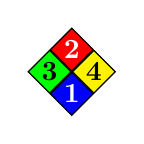
\begin{tikzpicture}	
  \node[fill=blue,shape=diamond,inner sep=0.3mm,draw=black,text=white,text width={}, anchor=north] {\bf 1};
  \node[fill=red,shape=diamond,inner sep=0.3mm,draw=black,text=white,text width={}, anchor=south] {\bf 2};
	\node[fill=green,shape=diamond,inner sep=0.3mm,draw=black,text=black,text width={}, anchor=east] {\bf 3};
	\node[fill=yellow,shape=diamond,inner sep=0.3mm,draw=black,text=black,text width={}, anchor=west] {\bf 4};
\end{tikzpicture}
  };
	 \node[anchor = center] at (27mm,1mm){
  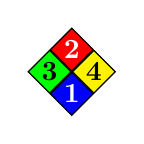
\begin{tikzpicture}	
  \node[fill=blue,shape=diamond,inner sep=0.3mm,draw=black,text=white,text width={}, anchor=north] {\bf 1};
  \node[fill=red,shape=diamond,inner sep=0.3mm,draw=black,text=white,text width={}, anchor=south] {\bf 2};
	\node[fill=green,shape=diamond,inner sep=0.3mm,draw=black,text=black,text width={}, anchor=east] {\bf 3};
	\node[fill=yellow,shape=diamond,inner sep=0.3mm,draw=black,text=black,text width={}, anchor=west] {\bf 4};
\end{tikzpicture}
  };
	 \node[anchor = center] at (40mm,1mm){
  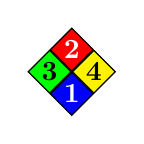
\begin{tikzpicture}	
  \node[fill=blue,shape=diamond,inner sep=0.3mm,draw=black,text=white,text width={}, anchor=north] {\bf 1};
  \node[fill=red,shape=diamond,inner sep=0.3mm,draw=black,text=white,text width={}, anchor=south] {\bf 2};
	\node[fill=green,shape=diamond,inner sep=0.3mm,draw=black,text=black,text width={}, anchor=east] {\bf 3};
	\node[fill=yellow,shape=diamond,inner sep=0.3mm,draw=black,text=black,text width={}, anchor=west] {\bf 4};
\end{tikzpicture}
  };
\end{tikzpicture}


\playercard{green}{Enforcer (South)}{\charisma{black}{1}}{\textit{LVL}}{\begin{tikzpicture}[fill opacity = 0](0,0)
%\coordinate[remember picture] (myorigin) at (0,0);
\node[anchor = south west] at (0,0) {\LevelStats{gray}{1}{}{2}{}{2}{}{3}};
\node[anchor = south west] at (11mm,0){\LevelStats{black}{2}{}{3}{}{4}{}{4}};
\node[anchor = south west] at (22mm,0){\LevelStats{gray}{3}{}{4}{}{4}{}{6}};
\node[anchor = south west] at (33mm,0){\LevelStats{black}{4}{}{6}{}{6}{}{8}};
\end{tikzpicture}}{Receive an additional {\inlinecost{black}{2}} at the beginning of each turn\\\ \\\textit{Hi!}}{}{}{C:/Users/Cake/Pictures/2015-08/cakeDerp.jpg};

\gearcard{black}{Lord Fluffington}{\cost{black}{3}}{}{Chain}{Must be Level 2 to equip}{\huge + {\GearStats{gray}{0}{}{2}{}{3}{}{1}}};

\smallgearcard{white}{Chain - Lord Fluffington}{\cost{black}{1}}{Must be Level 2 to equip.}{\huge + {\GearStats{gray}{0}{}{2}{}{3}{}{1}}}{C:/Users/Cake/Pictures/2015-08/cakeDerp.jpg}


\end{document}